\documentclass[fleqn,10pt,twoside]{gcb15submission}
\usepackage{url}\urlstyle{same}


\title{signalHsmm - a novel semi-Markov model of signal peptides}

\author[1]{Micha\l{}  Burdukiewicz}
\author[2]{Piotr Sobczyk}
\author[1]{Pawe\l{} B\l{}a\.{z}ej}
\author[1]{Pawe\l{} Mackiewicz}
\affil[1]{University of Wroc\l{}aw, Department of Genomics, Poland}
\affil[2]{Wroc\l{}aw University of Technology, Department of Mathematics, Poland}

\keywords{Keyword1, Keyword2, Keyword3}

\begin{abstract}
The proper localization of proteins in a cell is essential to perform their desired function. Information about the protein destination is included within the very protein in the form of short peptides called targeting signals. Ones of them are signal peptides, diverse N-terminal sequences, which are responsible for targeting of proteins to endomembrane system and their export outside the cell. Proteins equipped with signal peptides constitute a substantial fraction of the whole proteome and play crucial roles in metabolism, maintenance of tissue structure, immune response and regulation of other organismal functions. Moreover, the transport of proteins through the endomembrane system is important for their correct folding and posttranslational modifications. A common model of classical signal peptides assumes that they start with a positively charged n-region, followed by a hydrophobic h-region and a c-region ended with a cleavage site recognised by a signal peptidase.

However, our studies of many protein sequences representing the wide range of diversified taxonomic organisms indicate a variability of signal peptides. Therefore, the main goal of the study is to design a new probabilistic model for signal peptides, which will include knowledge about their organization, amino acid composition and variation.

The proposed model will be based on hidden semi-Markov models (HSMMs) and use intrinsic knowledge about signal peptides. The big advantage of the algorithm is a possibility to incorporate unique regions in the architecture of signal peptides. Therefore, HSMMs can be useful in recognition of atypical and artificial signal peptides. An aggregation of amino acids into physicochemical groups using the neural gas algorithm with k-fold cross-validation will reduce dimensionality of the problem and enable to learn the algorithm even on smaller data sets. The reduction will allow to use more complex probabilistic models and models specialized in the detection of signal peptides in different taxonomic groups of organisms, which improve the efficiency of the whole predictor. The n-gram and position-specific weight matrix methods will add more details to the probabilistic model.

Our preliminary model has showed the largest AUC=0.98 in comparison to other software and appeared very stable in the recovery of signal peptides after training even on very small data sets. Thanks to that, our model does not need to be permanently retrained with the continuous expansion of sequence databases. It should be emphasised that our model describes signal peptides from medically significant malaria parasites Plasmodium and their relatives (AUC = 0.92) more accurately than popular programs (0.84).

\end{abstract}

\begin{document}
\flushbottom
\maketitle
\thispagestyle{empty}


\section*{Introduction}

Your introduction goes here.
Some examples of commonly used {\LaTeX} commands and features are listed below, to help you get started.

All \textbf{accepted} submissions will be published as a \textbf{preprint collection} with \textbf{PeerJ} (\url{http://www.peerj.com}).
It will be clearly visible that the work
\begin{enumerate}
\item is a preprint (although reviewed and accepted by the GCB program committee)
\item has been presented at GCB'15
\end{enumerate}
by including a special GCB logo in the final version

If you decide to submit a full version after GCB to PeerJ or to PeerJ Computer Science, the procedure is very easy.
Of course, you are free to submit your paper to any other journal that allows existing preprints.


\subsection*{About PeerJ}

PeerJ is an award-winning open access publisher covering both computer science and the biological and medical sciences. 
PeerJ provides authors with three publication venues: PeerJ and PeerJ Computer Science (peer-reviewed academic journals) and PeerJ PrePrints (a 'pre-print server'). See \url{https://peerj.com/about/publications/} for more information.

The PeerJ model allows an author to publish articles in their peer-reviewed journal via the purchase of a lifetime Publication Plan. Prices start from just \$99 (a one-off payment) which entitles an author to the lifetime ability to publish 1 article per year for free.
The fee applies to all authors of an article, which encourages a reasonable number of co-authors and is generally less than for other open-access publishers.


\section*{Some \LaTeX{} Examples}
\label{sec:examples}

Use section and subsection commands to organize your document. \LaTeX{} handles all the formatting and numbering automatically. Use ref and label commands for cross-references.

\subsection*{Figures and Tables}

Use the table environment and the tabular command for basic tables --- see Table~\ref{tab:widgets}, for example.

To include a figure in your document, use the figure environment and the includegraphics command as in the code for Figure~\ref{fig:uaruhr}.

\begin{figure}[ht]\centering

\includegraphics[width=0.6\textwidth]{uaruhr}
\caption{An example image.}
\label{fig:uaruhr}
\end{figure}

\begin{table}[ht]
\centering
\begin{tabular}{l|r}
Item & Quantity \\\hline
Widgets & 42 \\
Gadgets & 13
\end{tabular}
\caption{\label{tab:widgets}An example table.}
\end{table}

\subsection*{Citations}

LaTeX formats citations and references automatically using the bibliography records in your .bib file.
Use the \verb|\cite| command for an inline citation, like \cite{MuellerRahmann+2003RobustEstimation}, and the \verb|\citep| command for a citation in parentheses \citep{MuellerRahmann+2003RobustEstimation}.

\subsection*{Mathematics}

\LaTeX{} is great at typesetting mathematics. Let $X_1, X_2, \ldots, X_n$ be a sequence of independent and identically distributed random variables with $\text{E}[X_i] = \mu$ and $\text{Var}[X_i] = \sigma^2 < \infty$, and let
$$S_n = \frac{X_1 + X_2 + \cdots + X_n}{n}
      = \frac{1}{n}\sum_{i}^{n} X_i$$
denote their mean. Then as $n$ approaches infinity, the random variables $\sqrt{n}(S_n - \mu)$ converge in distribution to a normal $\mathcal{N}(0, \sigma^2)$.

\subsection*{Lists}

You can make lists with automatic numbering \dots

\begin{enumerate}[noitemsep] 
\item Like this,
\item and like this.
\end{enumerate}
\dots or bullet points \dots
\begin{itemize}[noitemsep] 
\item Like this,
\item and like this.
\end{itemize}
\dots or with words and descriptions \dots
\begin{description}
\item[Word] Definition
\item[Concept] Explanation
\item[Idea] Text
\end{description}



\section*{Methods}

In a bioinformatics paper, the methods section should be the most important one.
Therefore, feel free to have more than one method section or to choose a more meaningful title for it.


\subsection*{Data selection}

Eukaryotic protein sequences and their annotations were properly prepared according to the literature of the subject and downloaded from UniProt database release 2015\_06. The positive set contained 2589 sequences with an experimentally confirmed signal peptide and its cleavage site. Sequences with more than one cleavage site were excluded from the final data set. The negative set comprised 152272 sequences without any signal peptide. Protein sequences with ambiguous symbols: X, J, Z and B were removed from the final sets. Proteins with selenocysteine (U) were also excluded from data set, because there are no records of signal peptides containing this amino acid.

\subsection*{Clustering of amino acids}

AAIndex


\subsection*{Subsection}

Here is an interesting equation that may be helpful in some situations:
\begin{equation}
\cos^3 \theta =\frac{1}{4}\cos\theta+\frac{3}{4}\cos 3\theta
\label{eq:refname2}
\end{equation}

\paragraph{Paragraph}
Nothing to see here. Move on.

\paragraph{Paragraph}
Really.
See Figure~\ref{fig:results} for more interesting results.

\begin{figure}[ht]\centering
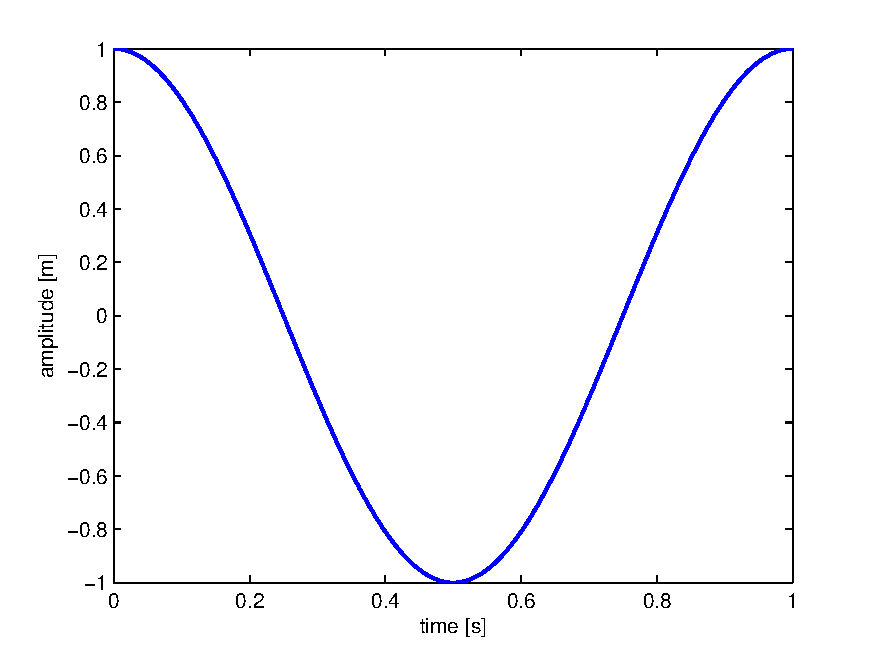
\includegraphics[width=0.6\textwidth]{results}
\caption{Can you guess which function this is?}
\label{fig:results}
\end{figure}



\section*{Results and Discussion}

You may want to separate results, discussion and conclusion, according to your needs.

Please submit the final pdf file via EasyChair to the GCB'15 program committee by June 30, 2015. 


\section*{Acknowledgments}
Thank you for your support!


\bibliography{sample}

\end{document}
